% !TEX root = thesis-main.tex


\chapter{Background}
\label{chapter:background} \label{nmtsec}

Neural machine translation (NMT) is an end-to-end learning approach to machine translation that is based on neural networks.
In contrast to traditional translation systems such as phrase-based machine translation (PBMT) \citep{koehn-etal-2003-statistical}, all components of the neural translation model are trained jointly to maximize translation performance.
In this chapter, we discuss the NMT paradigm and the properties of building a translation model.

The training data, in the format of parallel data, is a fundamental part of building NMT models.
We first explain the training data used in the NMT paradigm in Section~\ref{databg}, followed by an overview of data preparation and building the translation vocabulary in Section~\ref{bgvocab}.
Next, we discuss different word representation models in Section~\ref{bgemb}. 
In the following sections, we review the two main NMT frameworks used in this thesis: recurrent neural networks (Section~\ref{RNN}) and the transformer model (Section~\ref{TRNN}). 
Both models are classes of artificial neural networks and use large amounts of parallel data to learn a translation model. 
Finally, in Section~\ref{bgexp}, we describe the evaluation approaches used in the later chapters of this thesis. 

\section{Parallel and monolingual corpora} \label{databg}

Neural models, and specifically neural translation models, rely heavily on training data. 
The primary training data for learning translation models are parallel corpora, which are aligned texts in two or more languages. 
These corpora are often paired at the sentence-level, ideally providing an exact translation of every sentence in the source and target language. 

The quality of the translation system depends on the quality and the size of the training data. 
Acquiring good-quality parallel corpora requires manual translation by professional translators and as a result is expensive.
Examples of available parallel corpora gathered by experts in the domain include Europarl
\citep{koehn2005europarl}, which is the proceedings of the European Parliament published on the web, and JRC-Acquis 
\citep{steinberger2006jrc}, which is the total body of the European Union law applicable in the EU Member States.
\citet{callisonburch-EtAl:2007:WMT} gathered News Commentary corpora which consist of political and economic commentary crawled from the web site Project Syndicate.
This data is extracted every year for the translation task of the WMT conference \citep{barrault-EtAl:2019:WMT}. 

Monolingual data, in comparison, are available in abundance for many languages. 
Phrase-based machine translation models use monolingual corpora in the target language \citep{koehn-etal-2003-statistical, brants-etal-2007-large, koehn-etal-2007-moses} to improve the fluency of the generated translation \citep{lembersky-etal-2011-language}. 
Monolingual parallel corpora of aligned complex-simple sentences are also used with pharse-based \citep{wubben-etal-2012-sentence,kajiwara-komachi-2016-building} and neural \citep{zhang-lapata-2017-sentence} models to learn to simplify text.
The monolingual News Crawl corpus from WMT and many available corpora in the Linguistic Data Consortium (LDC)\footnote{\url{https://www.ldc.upenn.edu/}} are examples of commonly utilized data in machine translation.

Vanilla NMT models typically do not use any monolingual data in their training. 
In Chapters~\ref{chapter:research-02} and~\ref{chapter:research-03} of this thesis, we address this matter by focusing on the use of monolingual data for NMT.
Recently there have been studies that propose various approaches for incorporating information from monolingual data in the models \citep{domhan-hieber-2017-using,burlot-yvon-2018-using,currey-heafield-2019-zero}. 
\citet{currey2017copied} created a parallel corpus from monolingual data in the target language by copying it so that each source sentence is identical to its corresponding target sentence. With this simple technique, they observe improvements on relatively low-resource language pairs.
Another category of approaches is to translate sentences from monolingual data and augment the bitext with the resulting pseudo parallel corpora. 
This category of approaches is discussed in the following section.

\subsection{Back-Translation in machine translation} \label{bgbtref}

In this section, we introduce the conventional method of generating synthetic data, namely back-translation and its effectiveness in PBMT and NMT.
Back-translation uses an intermediate MT model, trained on parallel data, to translate target monolingual data into the source language.
The result of back-translation is a parallel corpus where the source side is synthetic MT output while the target is actual text written by humans.

This technique is not bounded to neural networks, and prior to NMT models, it has been used in combination with PBMT. 
\citet{Schwenk2008InvestigationsOL} proposes to translate large amounts of monolingual data with a PBMT system and use those as additional training data. They observe that this lightly-supervised training achieves improvements in translation quality.
\citet{Rapp:2009:BSA:1667583.1667625} introduces the back-translation score as an alternative mean for the evaluation of PBMT models.
He trains a translation model in both directions and evaluates the quality of the model by translating the target sentences back to the source language. 
The score is therefore computed by comparing the back-translated sentence to the original source sentence. 
As part of their experiments, \citet{tiedemann-etal-2016-phrase} note that back-translating sentences from monolingual news data and augmenting the parallel training data improves the translation quality of a PBMT system. 
In these experiments, the models have to be re-tuned from scratch with the additional synthetic data.

In the framework of NMT, \citet{sennrich-haddow-birch:2016:P16-11} show that back-translating sentences from monolingual data improves the performance of NMT models. 
This approach of augmenting the training data has since become common practice in training NMT models. 
\citet{pham2017karlsruhe} experimented with using domain adaptation methods to select monolingual data for back-translation based on the cross-entropy between monolingual data and the in-domain corpus \citep{axelrod2015class}, 
but did not find any improvements over random sampling as initially proposed by \citet{sennrich-haddow-birch:2016:P16-11}.

\citet{edunov-etal-2018-understanding} investigate back-translation in NMT at a large scale by adding hundreds of millions of back-translated sentences to the bitext.
They study different methods for generating synthetic sentences and show that synthetic data based on sampling and noised beam search provides a stronger training signal than using pure beam.
They observe that the generated corpora tend to stray away from the distribution of natural data.
\citet{brants-etal-2007-large} suggest a distributed language model infrastructure, which allows direct integration into the hypothesis-search algorithm.  
They observe that translation quality continues to improve with increasing language model size.
\citet{Ueffing2007} use an iterative procedure that translates the monolingual source language data in each iteration and then re-trains the phrased-based translation model.
They conclude that when bilingual training data are scarce, a PBMT system could be trained on a small amount of data and then iteratively improved by adding reliable translations of monolingual data to the training data. 

\citet{NIPS2016_6469} observe that any machine translation task has a dual task, for instance, English$\rightarrow$French translation (primal) versus French$\rightarrow$English translation (dual). 
They propose an approach based on reinforcement learning, where two agents, representing the primal and dual task, teach each other. 
The agents leverage monolingual data by translating it forward to the other language and then translate backward to the original language.
\citet{gulcehre2017integrating} propose two methods, shallow and deep fusion, for integrating a neural language model into an NMT system.
They observe improvements by combining the scores of a neural language model trained on target monolingual data with an NMT system.


\section{Translation vocabulary} \label{bgvocab}

In translation models, the vocabulary of the source and target language is defined as what the model is exposed to during training. 
Word-level translation models are unable to translate or generate unseen words at inference.
The number of words in the vocabulary can be remarkably large and training models on large vocabularies is computationally expensive.  

An early practice was to limit the vocabulary to the $K$ most frequent words, where $K$ is often in the range of 30k \citep{DBLP:journals/corr/BahdanauCB14} to 80k \citep{sutskever2014sequence}.
The tail of the vocabulary not included in this shortlist is mapped to a special token \texttt{[unk]} representing an unknown or out-of-vocabulary word.
This method results in neural models that can be trained and tested within a reasonable amount of time, however, as a consequence of this simplification, the translation quality of the model suffers. 
Specifically, the performance decreases significantly when the translation of a source sentence requires many unknown words \citep{cho2014properties}.

To address this issue, \citet{jean-etal-2015-using} proposed an approximate training algorithm that can use a very large target vocabulary (vocabularies of 500,000 source and target words). 
They show that decoding the target sentence by sampling only a small subset of the whole vocabulary achieves competitive results without sacrificing too much speed.
\citet{luong2014addressing} proposed a copy mechanism that aligns the OOV words on both the source and the target side by learning to copy indices.
\citet{sennrich-haddow-birch:2016:P16-12} analyzed NMT models that work with subword units and observed that the majority of tokens are potentially translatable through smaller units. 
They modify Byte Pair Encoding (BPE) \citep{10.5555/177910.177914} to segment words into subword units, where each of which should be frequently observed in the corpus. 
While some segmentations correspond to correct morphemes, for many words that is not the case. 
For instance, the word \textit{`quixotism'} would be segmented into \textit{`quixot + -ism'} and the word \textit{`sceptical'} would be segmented into \textit{`scep + -tic + -al'}.
This approach is very effective in generalization and is able to generate words not seen during training using these subword units.

In this thesis, we segment words during preprocessing using the BPE technique in all translation experiments unless stated otherwise.
We refer to the subword units throughout the chapters as \textit{tokens}. 

\section{Word representations} \label{bgemb} 

The first step in using neural models for text is to map the words in the vocabulary to \textit{dense vectors} of real numbers.
These vectors are somewhat similar to \textit{sparse vectors} used in distributional semantics, where they represent meaning by capturing similarities between lexical units based on their distributional properties \citep{baroni-etal-2014-dont,baroni-lenci-2010-distributional}.
The context of the lexical unit is commonly used for the computation of dense and sparse embeddings.
The intuition is that since similar words appear in similar contexts, they end up with similar embeddings \citep{firth1957synopsis}.
Computation of dense vectors is often a by-product of solving a natural language processing task such as language modeling or translation. 

Word representations can be categorized into two groups \citep{Wang2019UsingDE}: \textit{static embeddings} where a fixed vector is learned for each word in the vocabulary, and \textit{dynamic embeddings} where vectors are dynamically calculated for each sentence. 
In the next sections, we discuss different approaches in each category.

\subsection{Static embeddings}  \label{bgembstatic} 

Traditional word embedding techniques learn a global and static word embedding for every word in the vocabulary. 
\citet{mikolov2013efficient} proposed two models for learning word representations: continuous Skipgram and continuous bag-of-words (CBOW).
Both models use a feed-forward neural network architecture with the objective of modeling language, illustrated in Figure~\ref{bgsgcbowfig}.
This architecture does not include any non-linearity. 
\begin{figure}
\centering
\begin{subfigure}[t]{.45\textwidth}
  \centering
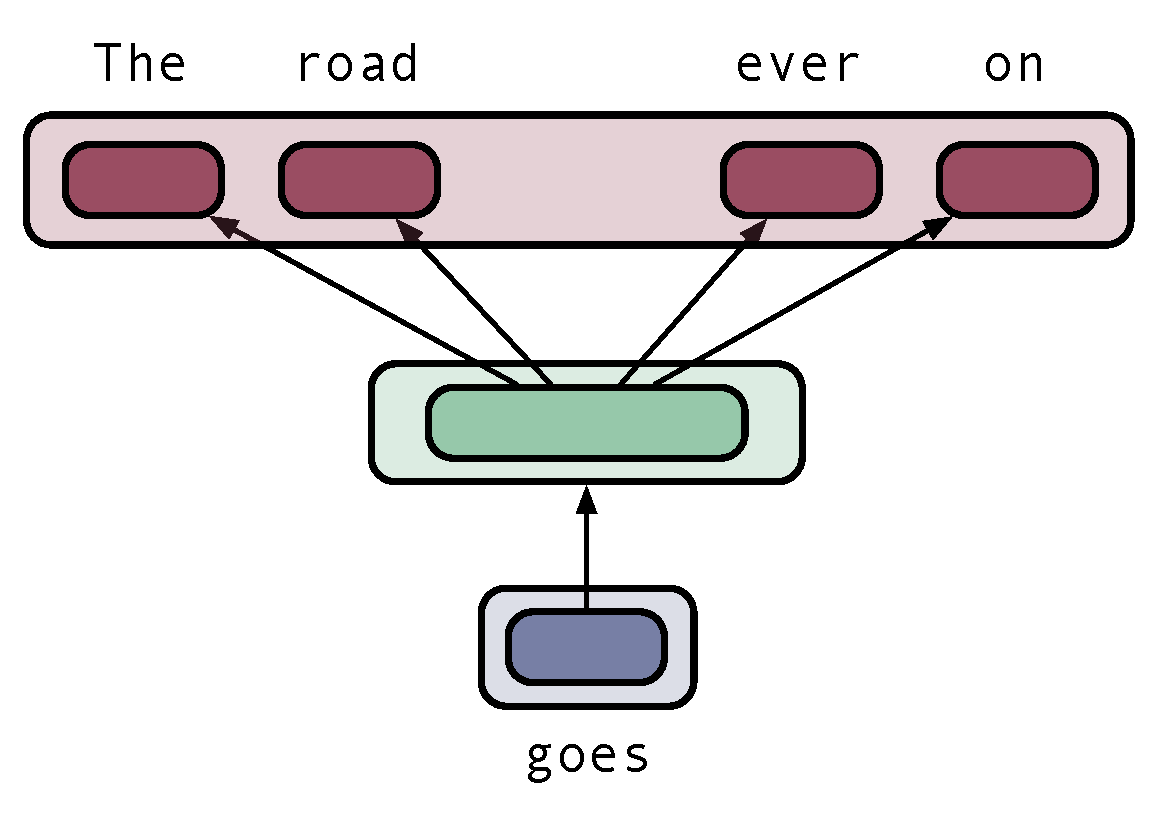
\includegraphics[width=0.8\linewidth]{02-background/figs/skipgram.pdf}
\caption{Skipgram model}
\label{bgsgfig}
\end{subfigure}%
\begin{subfigure}[t]{.45\textwidth}
  \centering
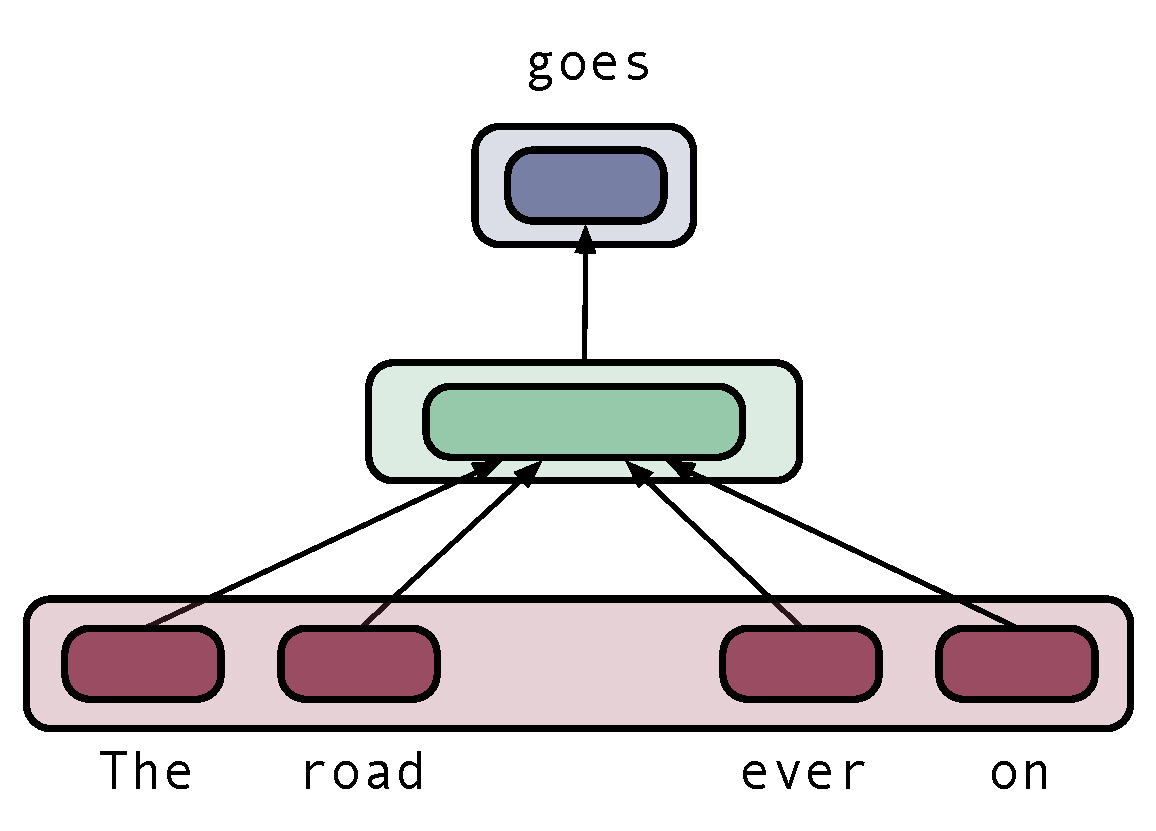
\includegraphics[width=.8\linewidth]{02-background/figs/cbow.pdf}
  \caption{CBOW model}
  \label{bgcbowfig}
\end{subfigure}
\caption{Representation learning architectures proposed by \citet{mikolov2013efficient}. The CBOW model predicts the current word given the context, and the Skipgram model predicts the surrounding words given the current word}
\label{bgsgcbowfig}
\end{figure}
The CBOW model has a projection layer which is shared between all words. This layer averages the input vectors.
Next, using a classifier, the model predicts the word $w_t$ given the context of words surrounding $w_t$ in a fixed sized window: $[w_{t-c}, \ldots, w_{t+c}]$. The objective of the CBOW model is to maximize the following average log probability:
\begin{align}
\frac{1}{T} \sum_{t=1}^T \log p(w_{t} \mid w_{t-c}, \ldots, w_{t-1}, w_{t+1}, \ldots, w_{t+c})
\end{align}

\noindent where $T$ is the length of the sequence of training words and $c$ is the context window size.
The Skipgram model is similar to CBOW, but instead of predicting $w_t$, the model predicts the words within a fixed range surrounding $w_t$.
The objective of the Skipgram model is to maximize the following average log probability:
\begin{align}
\frac{1}{T} \sum_{t=1}^T \sum_{\substack{-c \le j \le c \\ j \ne 0}} \log p(w_{t+j} \mid w_{t})
\end{align}

\noindent where $T$ is the length of the sequence of training words.
Note that in both CBOW and Skipgram models, the context window includes both the past and the future.

\citet{pennington2014glove} combined count-based matrix factorization and context-based Skipgram model together.
The intuition is that meaning of words can be captured by the ratios of co-occurrence probabilities.
They proposed a weighted least squares model that trains on global word co-occurrence counts. 
They showed that the vector space learned from this model captures meaningful vector space substructures.
While some syntactic and semantic features in language are captured by these word embeddings \citep{mikolov-etal-2013-linguistic}, the dimensions are often not interpretable. 

These models utilize surrounding words as context.
However, word representations can capture different phenomena if the definition of context is different. 
\citet{levy2014dependency} proposed to use dependency-based contexts, extracted from dependency parse-trees. 
They observed that these embeddings are less topical and exhibit more functional similarity than the original Skipgram embeddings.

Static embeddings for the most part learn a static matrix of embeddings for each word type and ignore capturing some nuances of language such as ambiguity. 
In Chapter~\ref{chapter:research-01}, we address this issue by exploring document topics and learning multiple embeddings per word type to capture polysemy. 

\subsection{Dynamic embeddings} 

Static models generate out-of-context embeddings for word types and are simple and efficient to train and use. 
However, learning meaningful word representations has recently been elevated beyond this paradigm. 
Rather than learning static representations for word types, these models learn \textit{dynamic} vectors for word instances in context using language modeling objectives. 
We denote this kind of embeddings as dynamic because instead of a static matrix of embeddings, they are obtained through the hidden states of a language model given the context.

\citet{peters-etal-2018-deep} proposed to use a bidirectional recurrent neural network to extract context-dependent representations.
The learning objective is to predict the next word in a sequence, given the previous context words. 
\citet{devlin-etal-2019-bert} use a transformer architecture and define two new objectives for training: \textit{masked language modeling}, and \textit{next sentence prediction}.
During masked language modeling, they mask a randomly selected word in a sentence, and the model has to predict that word given the context.
The second objective gets two input sentences and predicts whether the second sentence is indeed the next sentence.
The contextualized word embeddings are successful at downstream NLP tasks such as question answering and textual entailment \citep{zhang2019semanticsaware,garg2019tanda,Lan2020ALBERT:,mandar2020}.

While word vectors in neural translation models can be initialized with these static or dynamic word representations, they are often initialized randomly \citep{wu2016google}. 
One reason can be that with large-scale parallel data, these initial word representations will be forgotten during the training of the NMT model. 
\citet{qi-etal-2018-pre} showed that for low-resource language pairs and when languages are more similar, pre-trained embeddings can be effective.
\citet{lewis2019bart} recently proposed a denoising autoencoder model named BART for pretraining sequence-to-sequence models. 
They corrupt text with an arbitrary noising function and learn a model to reconstruct the original text.
BART is effective when fine-tuned for text generation and translation but also works well for comprehension tasks.
The research presented in this thesis mostly predates the work mentioned in this section.
We use \textit{static} embeddings in Chapter~\ref{chapter:research-01} where we investigate the effect of having more than one representation per word type. 
As for the chapters on machine translation, we consider the most widespread setup where embeddings are initialized randomly before training on the parallel data.

\section{Recurrent translation models} \label{RNN}

In this section, we discuss a category of neural models that are effective in modeling languages. 
Earlier developments of neural models addressing language modeling tasks incorporated the temporal structure of the language in the structure of the network \citep{Jacquemin1994ATC,Schmidhuber:HabilitationThesis}.  
A recurrent neural network (RNN) is an example of these sequential models \citep{10.5555/65669.104451}.
RNNs are powerful models that achieve state-of-the-art results in a variety of tasks such as question answering \citep{garg2019tanda}, reading comprehension \citep{Zhang2020RetrospectiveRF}, image semantic segmentation \citep{yuan2019objectcontextual}, and speech recognition \citep{8049322}. 

RNN models are capable of modeling sequences of text with various length, while selectively passing on information between different time steps in the sequence. 
A long short-term memory (LSTM) network \citep{hochreiter1997long} is an RNN structure that uses special LSTM units in addition to standard ones. 
These special units include a memory cell that can maintain information for long sequences.
LSTM models address the \textit{vanishing gradient problem} in the earlier RNN architecture where the weights and biases of the hidden layers are not updated effectively because the gradient decreases exponentially \citep{10.1142/S0218488598000094}. 

\begin{figure}[htb!]
\centering
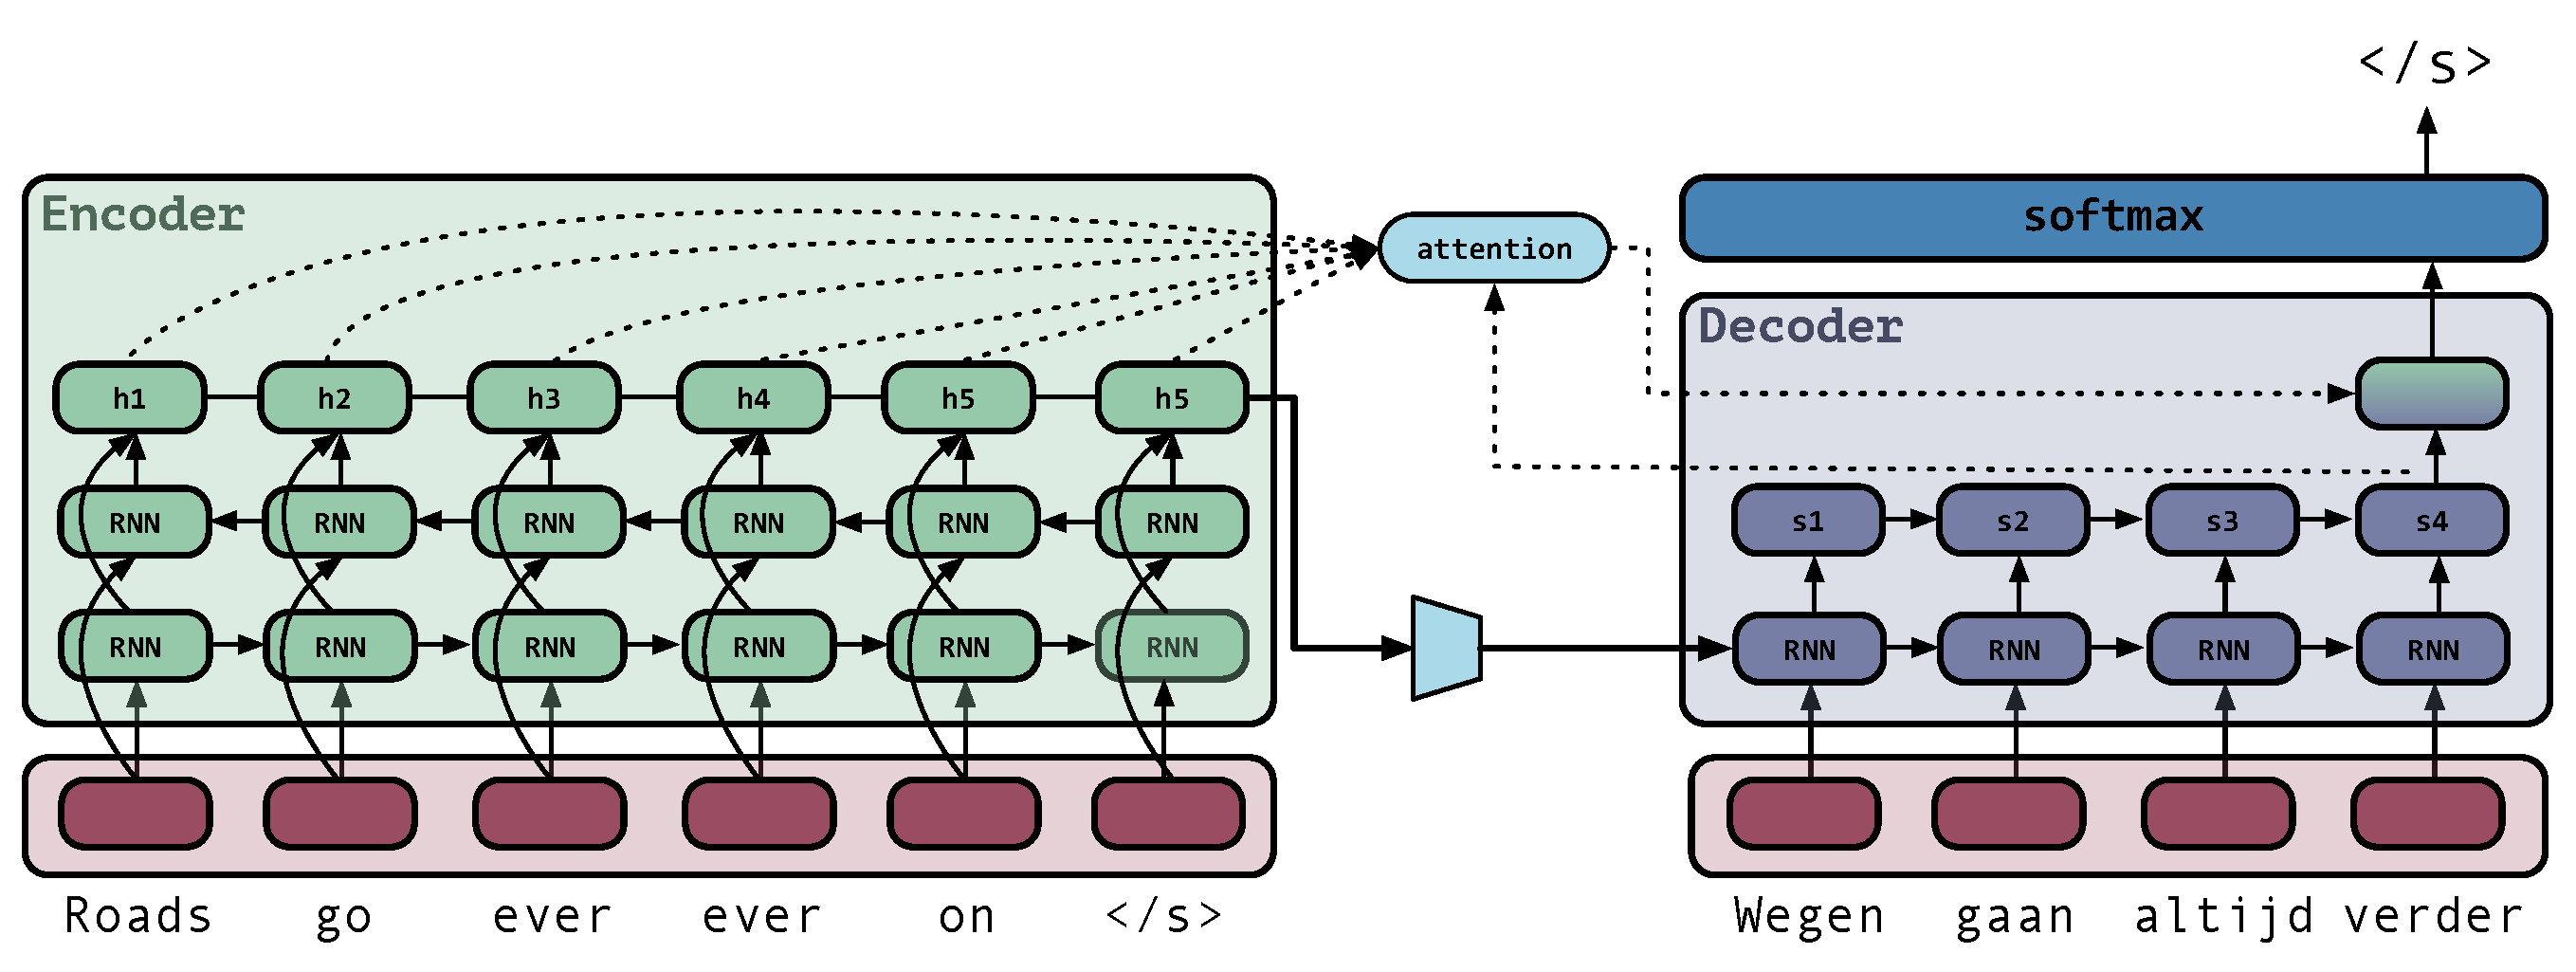
\includegraphics[width=0.95\linewidth]{02-background/figs/rnnarc.pdf}
\caption{An illustration of an RNN encoder-decoder with attention.}
\label{bgRNNfig}
\end{figure}

\citet{sutskever2014sequence} and \citet{cho2014properties} were among the firsts to employ RNNs to build an end-to-end machine translation model.
\citet{DBLP:journals/corr/BahdanauCB14} and \citet{luong:2015:EMNLP} introduced an \textit{attention mechanism} that achieved performance on par with traditional statistical models. 
In the following sections, we describe the RNN architecture with attention used in the NMT experiments in this thesis. 


\subsection{Model architecture}

Neural machine translation models fall under a sequence-to-sequence framework where an encoder builds up a representation of the source sentence and a decoder 
generates the target translation. 
Both the encoder and the decoder can be recurrent neural models.
Figure~\ref{bgRNNfig} illustrates this architecture which we will discuss in detail in this section. 
%
In order to train an NMT system, two sequences of tokens, $X =  \big[ x_1, \ldots, x_n \big] $ and $Y =  \big[ y_1, \ldots, y_m \big] $, are given in the source and target language, respectively.
As discussed in Section~\ref{bgemb}, the input tokens are mapped to an embedding space.
As a result, the source sequence is the input to the encoder as vectors: $\big[ \vt{x}_1, \ldots, \vt{x}_n \big]$.

The encoder then encodes the input sequence into hidden states, where at time step $t$ the hidden state is a function of the current input vector and the previous hidden state:
\begin{align}
\vt{h}_t = f(\vt{x}_t, \vt{h}_{t-1})
\end{align}

Function $f$ adds non-linearities to the transformation of the input sequence to the output of the encoder.
With a bidirectional architecture, two RNNs are run on the input sequence: one in forward and one in backward direction. The hidden state at time $t$ is created by concatenating the forward and backward hidden states
at each point in time, the input has access to the information on both sides. 
Note that the forward and backward hidden states are concatenated to create the top hidden states of the encoder, $\vt{h}_t$ as follows:
\begin{align}
\vt{h}_t = \big[ \overrightarrow{\vt{h}_t}^\intercal; \overleftarrow{\vt{h}_t}^\intercal \big]^\intercal,      t = 1, \ldots, n
\end{align}

%%%%%%%%%%%%%%%%%%

The decoder then generates the target translation one word at a time starting with the last hidden state of the encoder and the representation for the start-of-sentence symbol \mbox{\texttt{\textless s\textgreater}}.
Each decoder hidden state $\vt{s}_t$ is computed as:
\begin{align}
\vt{s}_t = g(\vt{s}_{t-1}, \vt{y}_{t-1}, \vt{c}_t)
\end{align}

\noindent where $g$ is a transformation function that outputs a vocabulary-sized vector and $\vt{y}_{t-1}$ is the representation of the previously predicted token.
$\vt{c}_i$ is the context vector for output at position $i$ and is defined as:
\begin{align}
\vt{c}_i = \sum_{j=1}^{n} \alpha_{ij} \vt{h}_j
\end{align}

This context vector is recomputed at each time step.
$\alpha_{ij}$ is the attention weight and it is computed for all source words at each time step $i$.
We will discuss different approaches to computing attention weights in Section~\ref{BGlstmATT}.

Next, the decoder predicts each target token $y_t$ by computing the conditional probability:
\begin{align}
p(y_t \mid y_{<t}, X) = \softmax \,(\vt{s}_t)
\end{align}

This conditional probability is computed over the vocabulary of the target language which is fixed during training and testing. 
For token $y_t$, the conditional probability $p(y_t \mid y_{<t}, X)$ during training quantifies the difficulty of predicting that token in the context $y_{<t}$.
The prediction loss of token $y_t$ is the negative log-likelihood of this probability.
During training on a parallel corpus $\mathbb{D}$, the cross-entropy objective function is defined as:
\begin{align}
\mathcal{L} = \sum_{(X,Y) \in \mathbb{D}} \sum_{i=1}^{m} - \log p(y_i \mid y_{<i}, X)
\end{align}

The objective of this function is to improve the model's estimation of predicting target words given the source sentence and the target context. 
The model is trained end-to-end by minimizing the negative log-likelihood of the target words using stochastic gradient descent.

NMT systems often benefit from multiple layers of stacked RNNs during training \citep{wu2016google}. 
By increasing the number of parameters, the learning capability of the model also increases \citep{britz-etal-2017-massive}.
\citet{belinkov-etal-2017-neural} show that different layers in the encoder capture different linguistic features, namely that higher layers capture semantics while lower layers tend to capture syntax.
Encoding the input sequence in both directions also provides advantages \citep{luong:2015:EMNLP,DBLP:journals/corr/BahdanauCB14}. The backward layer in a recurrent model learns more about the semantics of words, whereas the forward layer encodes more of the local context \citep{ghader-monz-2019-intrinsic}.

\subsection{Inference} \label{bgrnninference}

During inference, a trained model is given a source sentence and it generates the target translation word by word using a left-to-right beam search technique \citep{jelinek98}
This procedure was already adopted by pre-neural translation methods such as phrase-based translation models \citep{koehn-etal-2003-statistical}. 
Generation of target words stops when a special end-of-sentence symbol \mbox{\texttt{\textless /s\textgreater}} is generated. 
At each step, the model computes a probability distribution over all words in the target language and chooses the most likely word:
\begin{align}
\hat{Y} = \underset{Y}\argmax \; p({Y} \mid {X})
\end{align}

\citet{sutskever2014sequence} showed that increasing the beam size beyond 2 does not improve the predictions significantly and even with a beam size of 1, the model performs well. 
With a large enough beam size, the best translation performance can be reached with the drawback of efficiency \citep{freitag-al-onaizan-2017-beam}.
It is common practice to set beam size to around 5 to 10 \citep{wu2016google,edunov-etal-2018-understanding}.
Beam search decoding, even though effective, still suffers from \textit{exposure bias}.
Exposure bias results from the mismatch between how the models are trained and how they are used at inference \citep{wiseman-rush-2016-sequence,DBLP:journals/corr/RanzatoCAZ15}.
During training, the model is guided by the ground-truth target translation. 
However, at inference, target translations are not available and the model has to rely on its own predictions which can be wrong.
\citet{collobert2019a} proposed a fully differentiable beam search decoder that can be used during training and eliminates this bias.


\subsection{Attention mechanism} \label{BGlstmATT}

One of the shortcomings of the discussed models is that the translation quality decreases considerably as sentences become longer \citep{koehn2017six}.
One reason is that the source sentence is encoded into one \textit{fixed length} vector and this vector is expected to be a complete and static representation of the source sentence.
To address this problem, several works focus on learning a context vector with connections to the source sentence \citep{Graves2014NeuralTM,DBLP:journals/corr/BahdanauCB14,luong:2015:EMNLP}. 
This context vector regulates the alignment between the source and the target sentences and is a sum of the hidden states of the input, weighted by alignment scores.
At each time step $t$, the model computes a variable-length alignment weight vector based on the current target state and all source inputs. 
Table~\ref{backgroundattentions} summarizes different approaches for computing alignment scores.

\begin{table}
\centering
\small
\begin{tabularx}{0.93\linewidth}{lll}
 \toprule
\textbf{Name} & \textbf{Proposed by} & \textbf{Alignment score}  \\ \midrule
Additive & \citet{DBLP:journals/corr/BahdanauCB14} & $\text{score}(\vt{s}_i, \vt{h}_t) = \vt{v}^\intercal_a \tanh (\vt{W}_a[\vt{s}_i, \vt{h}_t])$ \\
 Location-base	 & \citet{luong:2015:EMNLP} & $\alpha_{n, t} = \softmax\,(\vt{W}_a\vt{s}_i) $ \\
General	 &  \citet{luong:2015:EMNLP} & $ \text{score}(\vt{s}_i, \vt{h}_t) = \vt{s}^\intercal_i  \vt{W}_a  \vt{h}_t $ \\
Dot-product	 &  \citet{luong:2015:EMNLP} & $\text{score}(\vt{s}_i, \vt{h}_t) = \vt{s}^\intercal_i \vt{h}_t  $ \\
 Scaled dot-product & \citet{vaswani2017attention} & $\text{score}(\vt{s}_i, \vt{h}_t) = \frac{\vt{s}^\intercal_i \vt{h}_t }{\sqrt{n}} $ \\
\bottomrule
\end{tabularx}
\caption{Different alignment scores in the literature used for creating the context vector. }
\label{backgroundattentions}
\end{table}

It is worth noting that while attention matches traditional word alignment at times, it often captures relations beyond that between the source and target sentence \citep{ghader-monz-2017-attention,koehn2017six}.



\section{Fully attention-based translation models} \label{TRNN}

In the previous section, we discussed attention mechanisms where the model selectively attends to the source sequence to make predictions. 
Self-attention is a type of attention mechanism that connects different positions \textit{within} a sequence to compute a representation.
The Transformer model proposed by \citet{vaswani2017attention} is a sequence-to-sequence model that relies solely on attention to encode the input and generate the output sequence. 
One of the main advantages of this architecture is that it can be trained with massive parallelization because it bypasses the recurrent dependency that exists in RNN models.  
The transformer model has been shown to perform quite well in bilingual and multilingual settings \citep{lakew-etal-2018-comparison} and has become the most common choice to implement NMT models \citep{edunov-etal-2018-understanding,aharoni-etal-2019-massively}.
In this section, we describe this architecture in more detail.

\subsection{Model architecture}


\begin{figure}
\centering
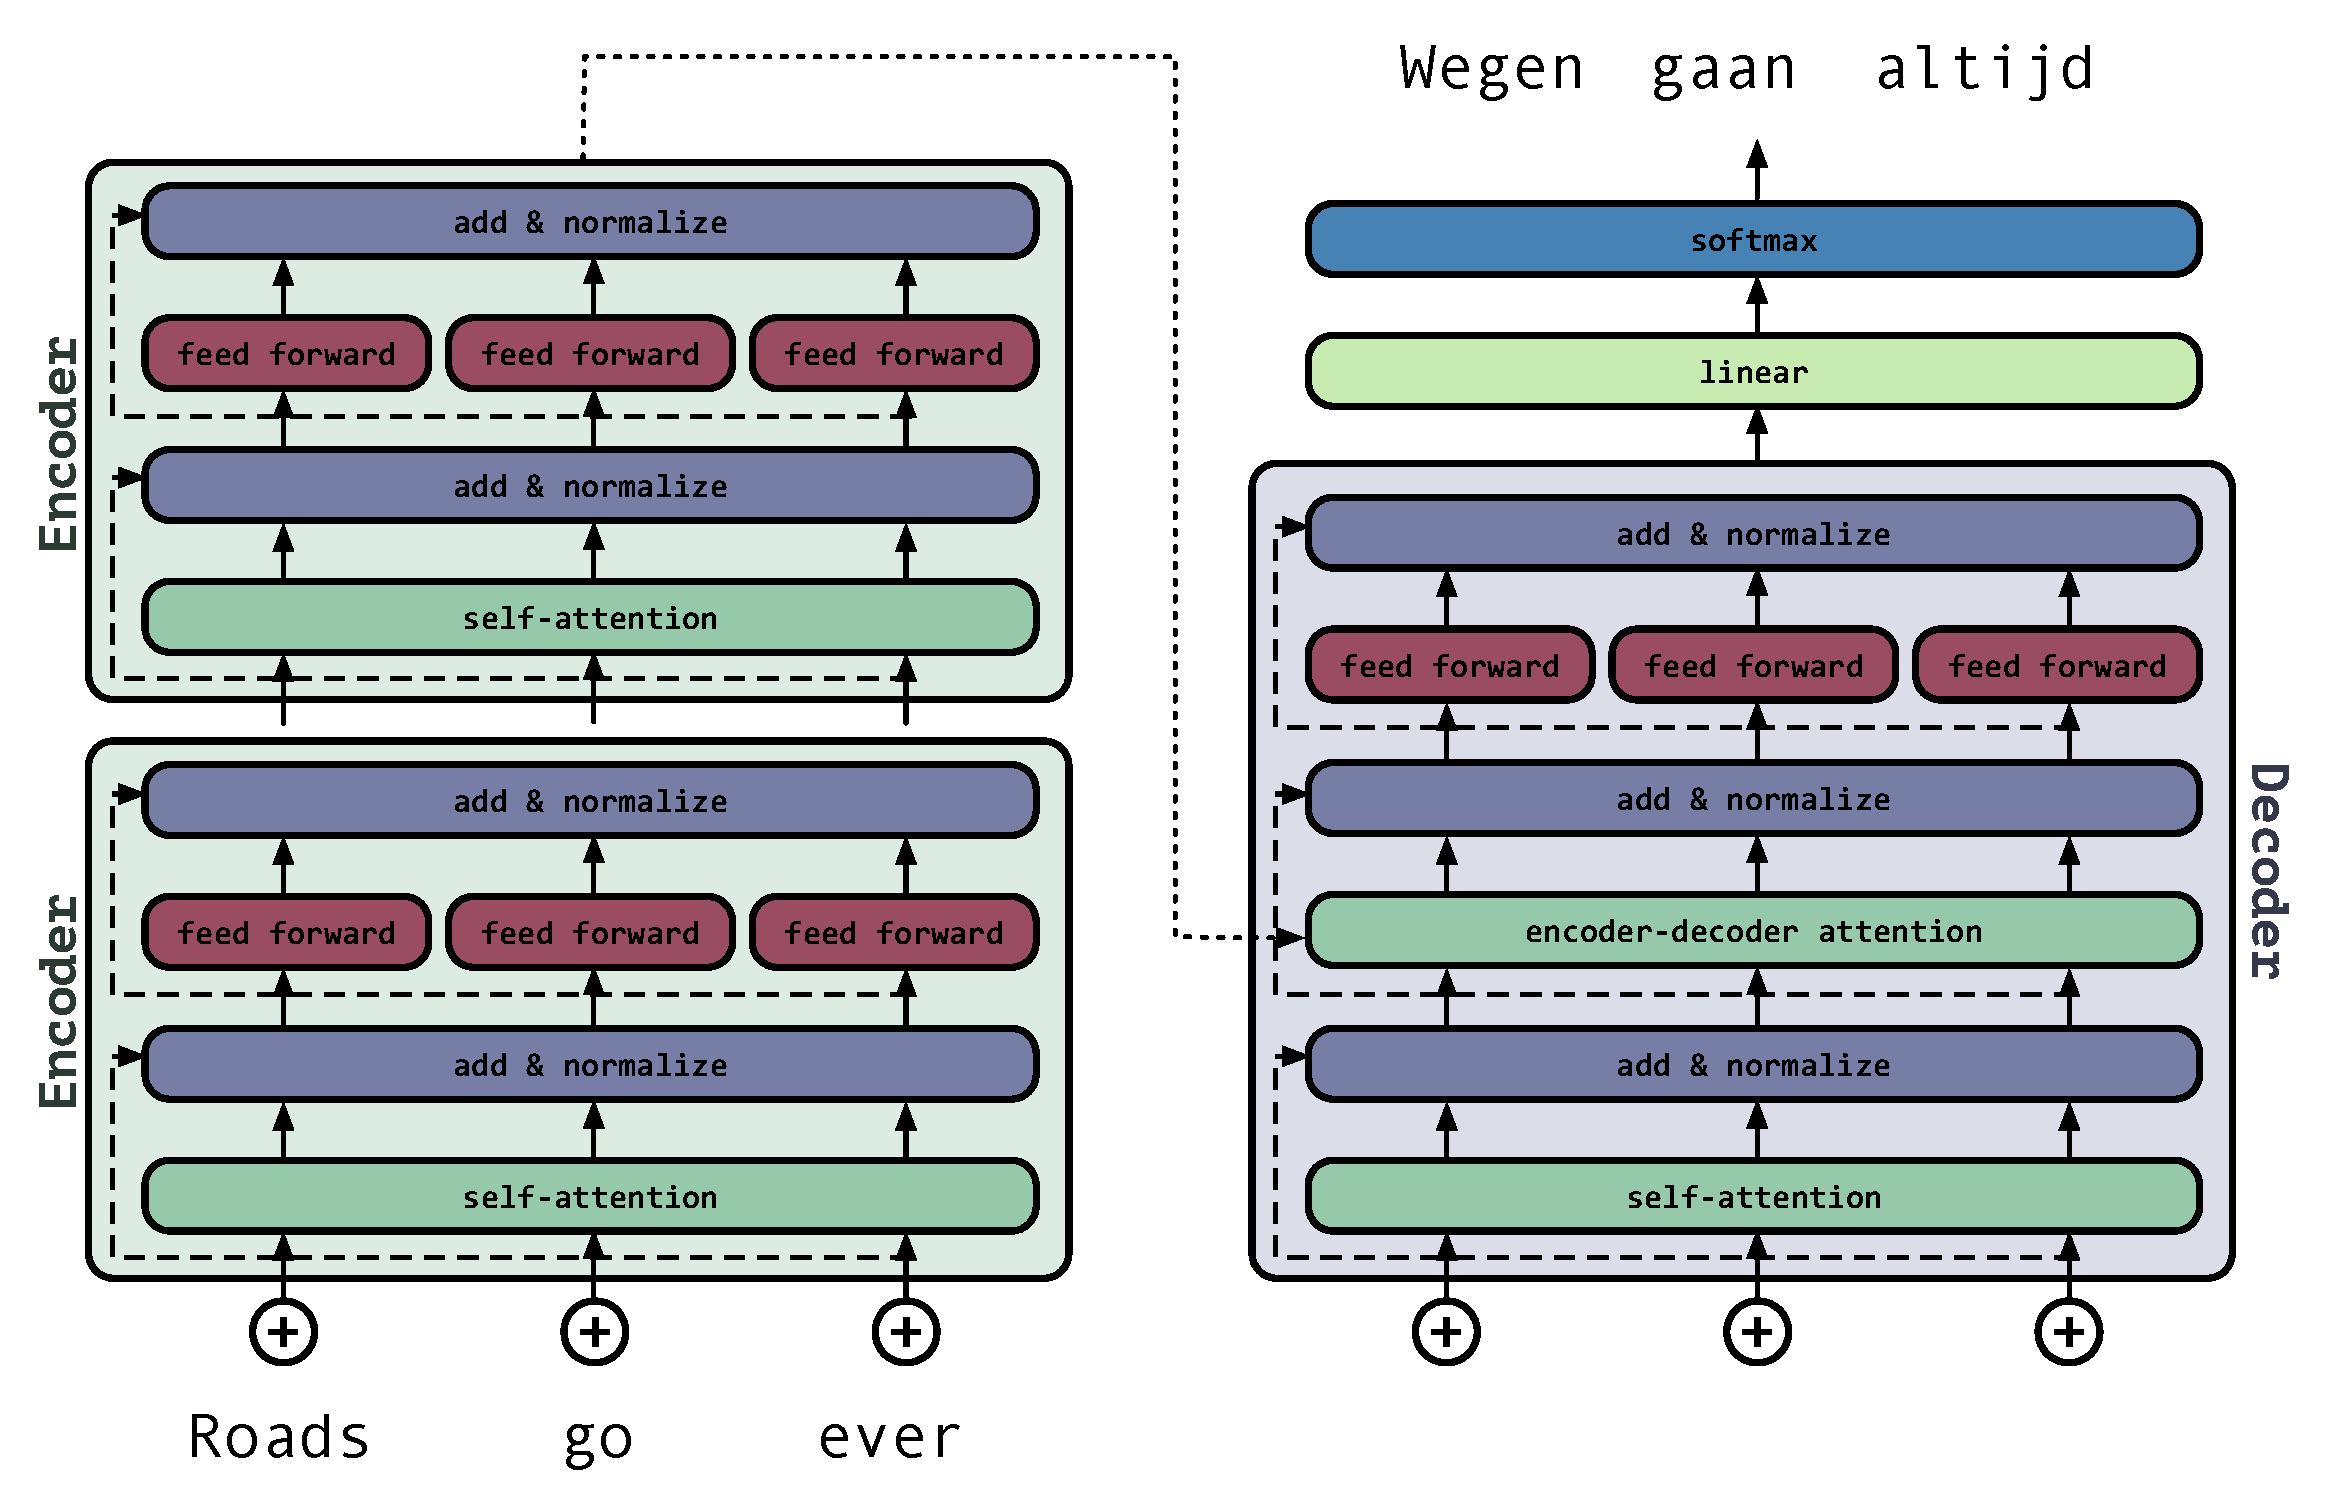
\includegraphics[width=0.95\linewidth]{02-background/figs/trnarc.pdf}
\caption{An illustration of a Transformer model introduced in \citet{vaswani2017attention}.}
\label{bgTRNfig}
\end{figure}

\begin{figure}
\centering
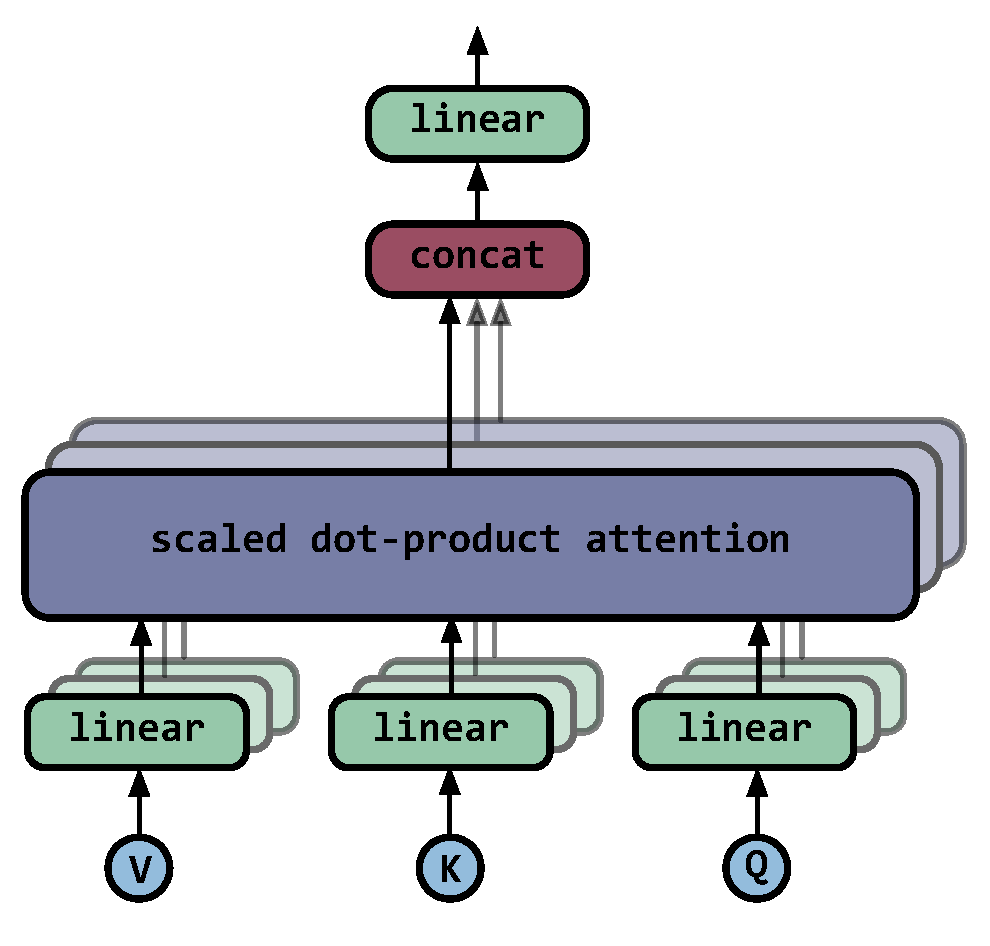
\includegraphics[width=0.5\linewidth]{02-background/figs/selfatt.pdf}
\caption{An illustration of self-attention in the Transformer model based on \citet{vaswani2017attention}.}
\label{bgTRNattfig}
\end{figure}


The transformer model is an encoder-decoder architecture without a sequential structure.
The encoder is given an input sequence of tokens $X = \big[ x_1, \ldots, x_n \big] $, and encodes it as a continuous representation $\vt{X} = \big[\vt{x}_1, \ldots, \vt{x}_n \big] $ based on the attention. 
The decoder then generates the output sequence $Y = \big[ y_1, \ldots, y_m \big] $ token by token, given the representation $\vt{X}$ and the previously generated token. 
Figure~\ref{bgTRNfig} illustrates this architecture which we will discuss in detail below. 

For every token $x_i$ in the input sequence, we first create a query $\vt{q}_i$, a key $\vt{k}_i$, and a value $\vt{v}_i$ vector.
Self-attention then uses \textit{scaled dot product attention} (last row in Table~\ref{backgroundattentions}) to compute the attention score of token $x_i$ against other words in the input sequence.
This attention has a scaling factor where $n$ is the dimension of the source hidden states.
To calculate representation $\vt{x}_i$, a softmax layer is then used to normalize the self-attention scores and multiplies it with $\vt{v}_i$.
In practice, the attention is computed on matrices of inputs ($\vt{Q}, \vt{K}, \vt{V}$) as follows:
\begin{align}
\attention (\vt{Q}, \vt{K}, \vt{V}) = \softmax (\frac{\vt{K}^\intercal \vt{Q} }{\sqrt{d_k}})\vt{V}
\end{align}

\noindent where $d_k$ is the embedding dimension of the key vectors which scales the dot product. The encoder is a stacking of identical layers each consisting of a \textit{multi-head self-attention} layer and a point-wise fully connected feed-forward network.
$\vt{Q}$, $\vt{K}$, and $\vt{V}$ matrices are split up into multiple heads and the multi-head attention mechanism computes the attention in parallel. 
Each token in the sequence goes through the encoder independently. 
During encoding, there are dependencies between the paths of different tokens in the self-attention layer, but the feed-forward layer of each token does not have any dependencies.
As a result words in the sequence can be processed in parallel. 
The independent attention outputs are then concatenated and linearly projected as follows: %transformed into expected dimensions.
\begin{align}
\text{Multi-Head Attention} (\vt{Q}, \vt{K}, \vt{V}) &= \concat (\text{head}_1, \ldots \text{head}_h) \vt{W}^o 
\end{align}
\noindent
where
\begin{align}
\text{head}_i = \attention(\vt{Q}\vt{W}_i^Q, \vt{K}\vt{W}_i^K, \vt{V}\vt{W}_i^V) 
\end{align}
\noindent
where $\vt{W}_i^Q, \vt{W}_i^K, \vt{W}_i^V$ are weight matrices that map the input representations to the query, key, and value matrices. $\vt{W}^o$ is the linear transformation that generates the output. 
All weight matrices are learned during training of the model.
Figure ~\ref{bgTRNattfig} illustrates this component. 
Similarly to the encoder, the decoder consists of a stack of identical layers, as well as a third sub-layer, which computes multi-head attention over the output of the encoder stack.
The self-attention layers in the decoder work slightly differently from the ones in the encoder. 
The computation of attention is \textit{masked} before the softmax step to prevent looking to the future of the sequence during training. 

Finally, there is a fully connected neural network that transforms the output of the stack of decoders into the target vocabulary vector.
The softmax function turns the scores into probabilities and the word with the highest probability is generated (greedy decoding). 
Alternatively, decoding can be done using the beam search technique similar to the RNN models discussed in Section~\ref{bgrnninference}.

\subsection{Residual connections} 

Another effective detail of the transformer architecture is the inclusion of residual connections \citep{He2016DeepRL} to facilitate optimization.
Residual connections connect the output of one layer with the input of an earlier layer.
Every self-attention and feed-forward neural network in the encoder and the decoder stack has a residual connection around it and a normalization layer \citep{Ba2016LayerN}.
This shortcut connection is particularly effective in training very deep architectures and mitigates the vanishing gradient problem. 

\subsection{Positional Encoding}

As discussed earlier, the transformer model does not have a recurrent structure and can be trained with a high degree of parallelization. 
However, languages are structured sequentially and it is necessary to encode some form of word order in the sequence \citep{tran-etal-2018-importance}. 
To address this shortcoming, the transformer adds a positional encoding vector to every word in the input sequence. 
These embeddings model the position of each word, or the relative distance between different words in the input.

\citet{vaswani2017attention} proposed sine and cosine functions of different frequencies to compute positional encodings:
\begin{align}
\text{positional encoding}_{(i, \delta)} = \begin{cases}
    \sin (\frac{i}{10000^{2\delta'/d}}) & \text{if $\delta = 2\delta'$}\\
        \\[5pt]
    \cos (\frac{i}{10000^{2\delta'/d}}) & \text{if $\delta = 2\delta' + 1$}
  \end{cases}
\end{align}

\noindent where $i$ is the position and $\delta = 1, \ldots, d$ is the dimension.
They also experimented with learned positional embeddings similar to \citet{pmlr-v70-gehring17a}, by assigning each input token with a learned vector that encodes its absolute position, and observed similar results to the sinusoidal version. 



\section{Translation evaluation} \label{bgexp}

We evaluate all translation experiments in this thesis using the BiLingual Evaluation Understudy metric, better known as BLEU \citep{Papineni2001}.
This metric assesses the closeness of the generated translation to a human reference translation.
It includes a \textit{brevity penalty} (BP) to avoid preferring shorter translations. 
The BLEU score for $n$-grams up to length $N$ is defined as:
%
\begin{align}
\bleu {_n} = \bp. \exp \bigg( \sum_{n=1}^N w_n \log p_n \bigg)
\end{align}

\noindent 
where $w_n$ is a weight assigned to the size of $n$-gram (often set uniformly to $1/N$). $p_n$ is computed as:
%
\begin{align} 
p_n &= \frac{ \sum\limits_{{c} \in \{candidates\}} \sum\limits_{{n\!\gram} \in {c}} \countop_{clip}({n\!\gram}) }{  \sum\limits_{{c'} \in \{candidates\}}^{} \sum\limits_{{n\!\gram }' \in {c'}} \countop({n\!\gram}')  }
\end{align}
\noindent
where:
\begin{align} 
\countop{_{clip}}(x) &= \min(\countop(x), \textit{max\_ref\_count})(x)) 
\end{align}
\noindent
Here, $candidates$ are translation candidates, and \textit{max\_ref\_count} is the largest count observed in the reference for that word. 
Scores are calculated over sentence pairs in the test set and the average BLEU is reported for the entire test set.  
Unless stated otherwise, in this thesis we compute case-sensitive BLEU up to and including $n$-grams of length 4. 

We also use other evaluation metrics, namely METEOR and Translation Error Rate (TER), in some chapters of this thesis.
METEOR is another metric to automatically evaluate translation quality \citep{banerjee-lavie-2005-meteor,denkowski-lavie-2011-meteor,denkowski:lavie:meteor-wmt:2014}.
Similar to BLEU, this metric compares the translation output with a reference translation, however, it addresses some of the deficiencies of the BLEU metric.
This is done by aligning the two sentences not only based on the exact match, but also on matching synonyms and paraphrases. 
METEOR has to be fine-tuned to achieve maximum correlation with human judgments \citep{agarwal-lavie-2008-meteor}.
TER is an easy-to-explain metric to compare translation output and manually created reference translation \citep{Snover06astudy}. 
It measures the number of edits required to change a translation output into one of the references.
A higher score of TER is a sign of more post-editing effort and it may not always correlate with translation quality.

While all these metrics attempt to measure translation quality, they assume inexact models of permissible variations in translation and may not capture the precise quality of a system \citep{callison-burch-etal-2006-evaluating}.
However, they allow for systematic evaluation of incremental changes to a single system and are very inexpensive to perform. 
We specifically choose BLEU because it is the most common metric and it makes it possible to compare various systems.
In Chapters~\ref{chapter:research-04} and~\ref{chapter:research-05} of this thesis, we explore cases where the translation quality of NMT models are affected, but individual automatic metrics do not reflect this change in quality. 

 


